%link do tworzenia tabeli https://tablesgenerator.com
%symbole matematyczne: https://oeis.org/wiki/List_of_LaTeX_mathematical_symbols
%narzedzia matematyczne: https://en.wikibooks.org/wiki/LaTeX/Mathematics
\documentclass{article}  %typ dokumentu
\usepackage[utf8]{inputenc} %rodzaj czcionki
\usepackage{geometry} %poprawienie marginesów
\usepackage{polski} %polskie znaki
\usepackage{multirow} %tabela
\usepackage{graphicx} %tabela
\usepackage{float} %tabela
\usepackage{diagbox} % 2 dane w jednym prostokącie
\usepackage{amsmath} % Matma
%\usepackage{blindtext} %
%\usepackage{enumitem}
\usepackage{tikz} %rysowanie
\usepackage{fancyhdr} %headery i footery
\usetikzlibrary{arrows}
\graphicspath{{pictures/}}
\geometry{margin=0.7in}


\pagestyle{fancy}
\fancyhf{}
%--------------------------------------------------------------
\def\tytul{Narzędzia pomiarowe} %<<<Tutaj wpisz tytuł ćwiczenia
%--------------------------------------------------------------
\begin{document}

\lhead{Miernictwo elektroniczne - \tytul}
\cfoot{\thepage}
\rhead{\thepage}
\begin{table}[H]
\centering
\resizebox{\textwidth}{!}{
\begin{tabular}{|c|c|c|}
\hline

\begin{tabular}[c]{@{}c@{}}Byczko Maciej\\Malek Jan\\Maziec Michał\end{tabular}&
\begin{tabular}[c]{@{}c@{}}Prowadzący:\\ Mgr Inż. Monika Prucnal\end{tabular} &
\begin{tabular}[c]{@{}c@{}}Numer ćwiczenia\\
%----------------------------------------
    1 %<<<tutaj wpisz numer ćwiczenia
%----------------------------------------
\end{tabular} \\ \hline
\begin{tabular}[c]{@{}c@{}}Grupa nr.\\
%----------------------------------------
    1 %<<<tutaj wpisz numer grupy
%----------------------------------------    
\end{tabular} & \begin{tabular}[c]{@{}c@{}}Temat ćwiczenia:\\\tytul
\end{tabular}&Ilość punktów: \\ \hline\begin{tabular}[c]{@{}c@{}}Tydzień Nieparzysty\\ Godzina 11:15-13:00\end{tabular}&\begin{tabular}[c]{@{}c@{}}Data wykonania ćwiczenia:\\
%----------------------------------------
16 marca 2020 %<<<tutaj wpisz datę
%----------------------------------------
\end{tabular} &\\ \hline\end{tabular}}\end{table}
% \begin{comment}
% w części teoretycznej należy zawrzeć tutaj krótki wstęp teoretyczny,spis przyrządów, opis przebiegu doświadczenia, najlepiej w punktach
% oblicznoe dokładności pomiarowe w tabelach, zaokrąglony przedział wyników pomiaru w tabelach, wykorzystane wzory, przykładowe obliczenia
% opisane rysunki,schematy pomiarowe, wnioski końcowe !!! UNIKAĆ PUSTYCH PRZESTRZENI!!!
% \end{comment}
\centering
\section{Część teoretyczna i opisowa}
\subsection{cel ćwiczenia}
\subsubsection{Wprowadzenie}
\begin{flushleft}
    Celem ćwiczenia jest poznanie źródeł informacji o parametrach i warunkach exploatacji narzędzi pomiarowych,\\
    zapoznanie ze sposobami użytkowania wybranych analogowych i cyfrowych przyrządów pomiarowych oraz wzorców rezystancji,
    nabycie umiejętności oceny niepewności wyników pomiarów, wynikającej z wartości błędów granicznych użytkowanego narzędzia pomiarowego.
\end{flushleft}
    \subsection{program ćwiczenia}
    \begin{enumerate}
        \item Przyrząd analogowy
        \begin{enumerate}
            \item Rozpoznać informacje umieszczone na podzielni przyrządu, 
            ze szczególnym uwzględnieniem parametrów metrologicznych i sposobem podawania informacji o błędzie podstawowym przyrządu.
            \item Zmierzyć wskazane napięcie woltomierzem magnetoelektrycznym. 
            Pomiar tego samego napięcia wykonać stosując różne zakresy woltomierza. Porównać wyniki pomiarów.
            \item Obliczyć  graniczne  błędy  bezwzględne  i  względne  wskazań  woltomierza  na  dla  każdego wyniku.
            \item Podać dla każdego pomiaru przedział wartości w jakim znajduje się napięcie wskazywane przez woltomierz. 
        \end{enumerate}
        \item Przyrząd cyfrowych
            \begin{enumerate}
                \item Zapoznać się parametrami metrologicznymi i technicznymi oraz sposobem podawania błędu podstawowego dla przyrządó cyfrowych.
                \item Zmierzyć wskazane napięcie. Pomiar tego samego napięcia  wykonać stosując różne zakresy woltomierza. Porównać wyniki pomiarów.
                \item Obliczyć graniczne błędy bezwzględne i względne wskazań woltomierza dla każdego wyniku.
                \item Podać dla każdego pomiaru przedział wartości w jakim znajduje się napięcie wskazywane przez woltomierz.
                \item Zmierzyć prąd płynący we wskazanym obwodzie. Pomiar wykonać stosując  różne zakresy amperomierza.
                \item Obliczyć graniczne błędy bezwzględne i względne wskazań amperomierza decydujące o niepewności wartości odczytanej z amperomierza.
            \end{enumerate}
        \item Wzorzec rezystancji
            \begin{enumerate}
                \item Zapoznać się z informacją umieszczoną na jednomiarowym wzorcu rezystancji i na dekadzie rezystancyjnej.
                \item Obliczyć błąd graniczny bezwzględny wzorca rezystancji i podać przedział wartości, w którym leży rzeczywista wartość wzorca.
                \item Zmierzyć omomierzem cyfrowym wartość rezystora wzorcowego oraz wartość rezystancji R ustawionej na dekadzie. 
                \item Określić błąd bezwzględny i względny wyniku pomiaru (niepewność  wyniku pomiaru) wynikający z błędu granicznego omomierza i 
                na tej podstawie przedział wartości, w którym znajduje się rzeczywista wartość mierzonej rezystancji. 
                \item Sprawdzić czy wyniki obliczeń z punktu 3.2 nie są sprzeczne z wynikami obliczeń w punktach 3.4.
            \end{enumerate}
    \end{enumerate}
\subsection{Wstęp teoretyczny}
\begin{flushleft}
    Do wykonania pomiaru niezbędne są narzędzia pomiarowe i pomocniczy sprzęt pomiarowy. 
    Do narzędzi pomiarowych zaliczane są przyrządy pomiarowe i wzorce miar. 
    Wartości błędów narzędzi pomiarowych bardzo rzadko są znane dokładnie. 
    Producenci aparatury podają jedynie wartości graniczne błędów podstawowych i dodatkowych, 
    gwarantując tym samym, że przy zachowaniu określonych warunków użytkowania danego narzędzia pomiarowego popełniane nim błędy nie przekroczą określonych wartości. 
    Błędy podstawowe narzędzi pomiarowych określają niedokładność wykonanego nimi pomiaru w warunkach odniesienia. 
    Warunki odniesienia stanowi odpowiedni, znormalizowany, zbiór określonych wartości wielkości wpływających (temperatury, wilgotności,...).
    Parametrem metrologicznym charakteryzującym narzędzie pomiarowe jest błąd podstawowy. 
    Błędy podstawowe wielu narzędzi pomiarowych podawane są w postaci odpowiedniego wskaźnika klasy dokładności.
\end{flushleft}
    \subsection{spis przyrządów}
\begin{table}[H]
    \centering
    \begin{tabular}{|l|l|l|l|}
    \hline
    Nr.&Przyrząd             & Nazwa    & Klasa przyrządu    \\ \hline
    1. &Zasilasz             & TYP 5121 &   ---------        \\ \hline
    2. &Woltomierz analogowy &          &      0.5           \\ \hline
    3. &Woltomierz cyfrowy   &          &   ---------        \\ \hline
    4. &Amperomierz analogowy&          &      0.5           \\ \hline
    5. &Amperomierz cyfrowy  &          &   ---------        \\ \hline
    6. &omomierz             &          &   ---------        \\ \hline
    \end{tabular}
    \end{table}


\subsection{przebieg ćwiczenia}
    \begin{itemize}
        \item podłączenie urządzenia do 
        \item 
        \item 
        \item 
    \end{itemize}
\subsection{wzory}
$\Delta U = \pm \frac{kl \ast U_z}{100}$

\section{Pomiary i obliczenia}
\subsection{Doświadczenie 1}
\subsubsection{Schemat pomiarowy}
    \begin{figure}[H]
        \centering
        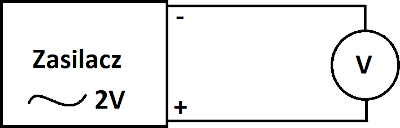
\includegraphics{zas-woltanal}
        \caption{schemat pomiarowy}
    \end{figure}
\subsubsection{Pomiary}
\begin{table}[H]
    \centering
    \resizebox{\textwidth}{!}{%
    \begin{tabular}{|c|c|c|c|}
    \hline
    Nr. pomiaru & Zakres pomiaru{[}V{]} & Wskazania podziałki{[}max. 75 działek{]} & Wyniki pomiaru{[}V{]} \\ \hline
    1. & 30  & 6  & 2.4  \\ \hline
    2. & 15  & 11 & 2.2  \\ \hline
    3. & 7.5 & 23 & 2.3  \\ \hline
    4. & 3   & 58 & 2.32 \\ \hline
    \end{tabular}%
    }
    \end{table}

\subsection{Obliczenia}
Brak obliczeń
\section{Wyniki i Wnioski}
Pomiary są dosyć niedokładne z powodu analogowego sposobu dokonywania pomiarów
\end{document}
